
\section*{CHƯƠNG 3. THIẾT KẾ HỆ THỐNG}
\setcounter{section}{3}
\setcounter{subsection}{0} %LƯU Ý MỖI LẦN THÊM CHƯƠNG MỚI CẦN THÊM CÂU NÀY ĐỂ RESET THỨ TỰ CỦA SUBSECTON VỀ 1
\setcounter{table}{0} % LƯU Ý SAU MỖI LẦN GỌI BẢNG HAY HÌNH ẢNH PHẢI THÊM CÂU NÀY ĐỂ RESET THỨ TỰ
\setcounter{figure}{0} %% LƯU Ý SAU MỖI LẦN GỌI BẢNG HAY HÌNH ẢNH PHẢI THÊM CÂU NÀY ĐỂ RESET THỨ TỰ
\addcontentsline{toc}{section}{\numberline{}CHƯƠNG 3. THIẾT KẾ HỆ THỐNG}

Đây là chương chúng em sẽ thực hiện thiết kế từ tổng quan đến chi tiết của hệ thống. Từ việc xây dựng sơ đồ kiến trúc hệ thống,
đến thiết kế từng chức năng cho cả ứng dụng di động, website và server, nội dung chủ yếu của chương sẽ xoay quanh các hình
ảnh và sơ đồ nhằm diễn tả chi tiết từng luồng hoạt động của hệ thống và cách các phần trong hệ thống tương tác với nhau.

\subsection{Sơ đồ kiến trúc hệ thống}
Hệ thống chúng em xây dựng được chia làm ba phần Device, Application và Server. Các chi tiết cụ thể được thể hiện trong
hình vẽ:

\begin{figure}[H]
  \centering
  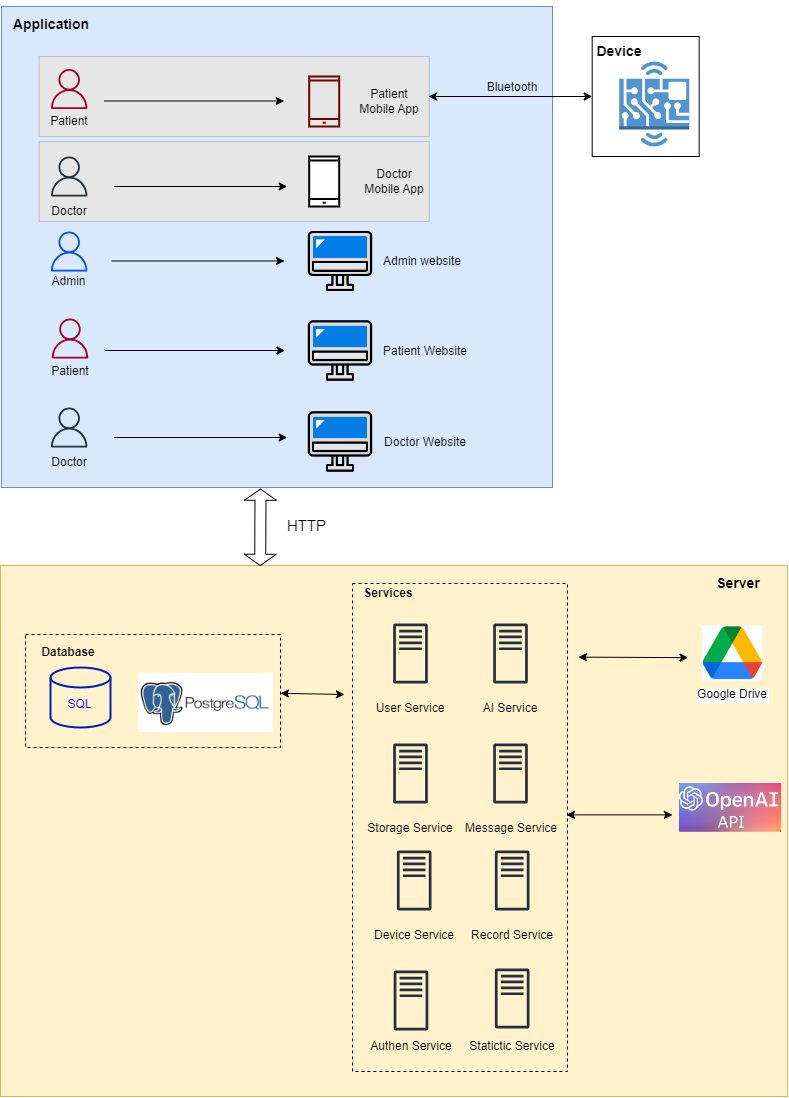
\includegraphics[width=12cm,height=10cm]{Images/system/fmECG_architecture-System_Architecture.png}
  \caption[Kiến trúc tổng quan hệ thống]{\bfseries \fontsize{12pt}{0pt}\selectfont Kiến trúc tổng quan hệ thống}
  \label{fmECG_architecture-System} %đặt tên cho ảnh
\end{figure}

Hình \ref{fmECG_architecture-System} thể hiện ba phần: 

\begin{adjustwidth}{1.5em}{}
\begin{itemize}
  \item Device: Thiết bị phần cứng đo điện tim, để kết nối với App bệnh nhân thông qua Bluetooth 
  \item Application: Bao gồm ứng dụng của bệnh nhân, ứng dụng của bác sĩ và Website của Admin
  \item Server: Bao gồm các Services để xử lý các yêu cầu gửi từ Application, cơ sở dữ liệu và Cloud lưu trữ
\end{itemize}
\end{adjustwidth}

Trong hệ thống thì Devices là phần mà chúng em sẽ không trực tiếp thực hiện trong đồ án này, Application và Server sẽ là
phần mà đồ án chúng em thực hiện. Ở trong sơ đồ kiến trúc hệ thống riêng có bệnh nhân sẽ có tương tác trực tiếp với Devices,
còn lại khối Application sẽ tương tác với Server thông qua API với giao thức HTTP. Khi nhận được yêu cầu từ Application,
Server sẽ thực hiện xử lý dữ liệu, mọi yêu cầu đến đều được xử lý bởi Services, tuỳ vào yêu cầu đến Services tương ứng sẽ đảm nhiệm 
việc lấy/lưu dữ liệu trong cơ sở dữ liệu sau đó trả ra kết quả cho người dùng.
\begin{adjustwidth}{1.5em}{}
\begin{itemize}
  \item User Services: Xử lý các yêu cầu liên quan đến người dùng như đăng ký, đăng nhập, lấy thông tin tài khoản
  \item ECG Services: Xử lý các tác vụ liên quan tới dữ liệu điện tim
  \item Storage Services: Xử lý các tác vụ lưu trữ dữ liệu của hệ thống với AWS
  \item Message Services: Xử lý các yêu cầu liên quan tới hội thoại, tin nhắn.
\end{itemize}
\end{adjustwidth}
Ngoài ra, hệ thống sẽ phải có kết nối bluetooth low energy giữa thiết bị đo và ứng dụng di động để có thể truyền/nhận dữ liệu.
Trên đây là tổng quan về kiến trúc hệ thống, phần tiếp dưới đây chúng em xin phép trình bày kỹ hơn về từng khối nhỏ hơn
dựa vào những đối tượng đã được xác định trong hệ thống.

\newpage
\subsection{Sơ đồ khối phần mềm}

\subsubsection{Ứng dụng di động cho bệnh nhân}
\mbox{}

\begin{figure}[H]
  \centering
  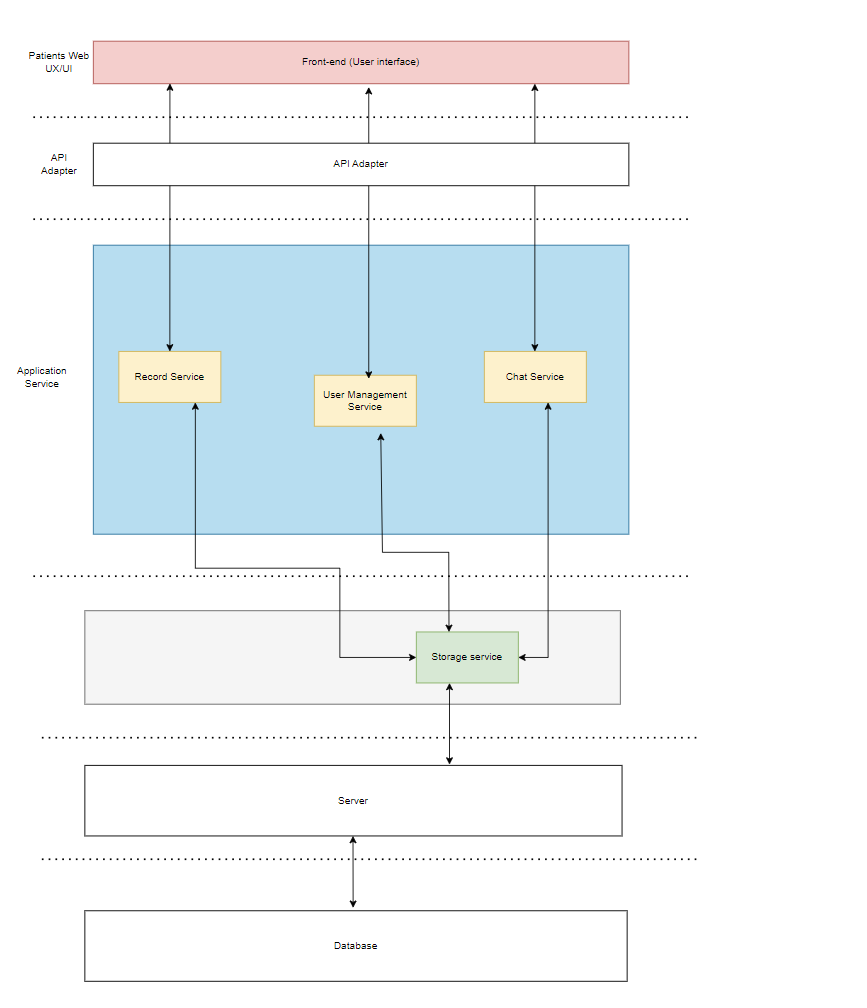
\includegraphics[width=15cm,height=15cm]{Images/system/fmECG_architecture-Patient.drawio.png}
  \caption[Sơ đồ khối cho App bệnh nhân]{\bfseries \fontsize{12pt}{0pt}\selectfont Sơ đồ khối cho App bệnh nhân}
  \label{fmECG_architecture-Patient} %đặt tên cho ảnh
\end{figure}

Trong hình trên, lớp trên cùng User interface là lớp để người dùng tương tác và thực hiện lời gọi thông qua API Adapter, 
các yêu cầu của người dùng sẽ được xử lý thông qua Services và phản hồi lại với người dùng qua giao diện. Dưới đây là phần
giải thích Services trong hình:
\begin{adjustwidth}{1.5em}{}
\begin{itemize}
  \item ECG Service: Khối có nhiệm vụ xử lý yêu cầu cho các trạng thái đo: thực hiện đo, kết thúc đo, lưu kết quả đo
  \item ECG Signal Processing Service: Khối có nhiệm vụ xử lý tín hiệu đo để phân tích sâu, hiển thị lên màn hình
  \item User Management Service: Khối có nhiệm vụ xử lý các vấn đề liên quan đến người dùng như đăng nhập, đăng ký
  \item Chat Service: Khối có nhiệm vụ quản lý việc chat, trao đổi thông tin
  \item Storage Service: Khối có nhiệm vụ lưu thông tin vào bộ nhớ
\end{itemize}
\end{adjustwidth}

Riêng với App cho bệnh nhân thì sẽ có Khối Bluetooth và Khối Device để phục vụ cho việc đo điện tim.
\subsubsection{Ứng dụng di động cho bác sĩ}

\begin{figure}[H]
  \centering
  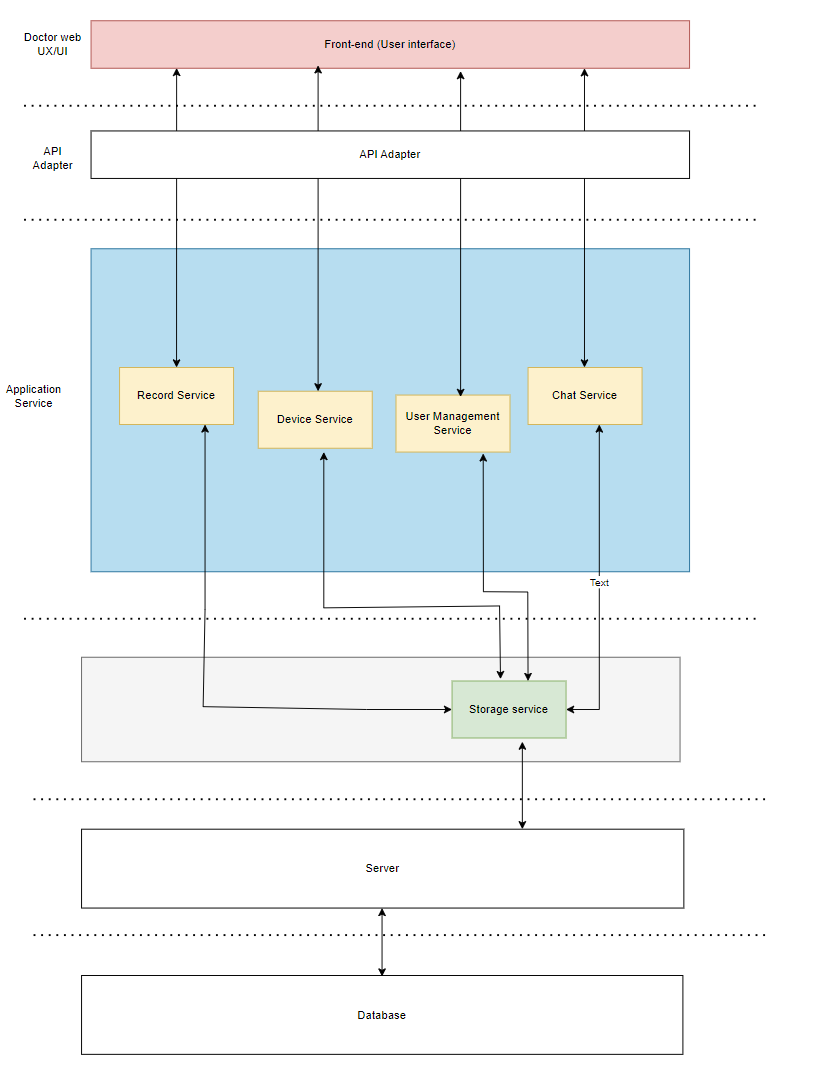
\includegraphics[width=12cm,height=14cm]{Images/system/fmECG_architecture-Doctors.drawio.png}
  \caption[Sơ đồ khói cho App bác sĩ]{\bfseries \fontsize{12pt}{0pt}\selectfont Sơ đồ khối cho App bác sĩ}
  \label{fmECG_architecture-Doctors} %đặt tên cho ảnh
\end{figure}

Về cơ bản, ứng dụng di động cho bác sĩ có những khối tương tự với bệnh nhân, trừ việc bác sĩ sẽ không có hai khối Device
và Bluetooth để phục vụ việc đo như bệnh nhân.


\subsubsection{Website cho quản trị viên}

\begin{figure}[H]
  \centering
  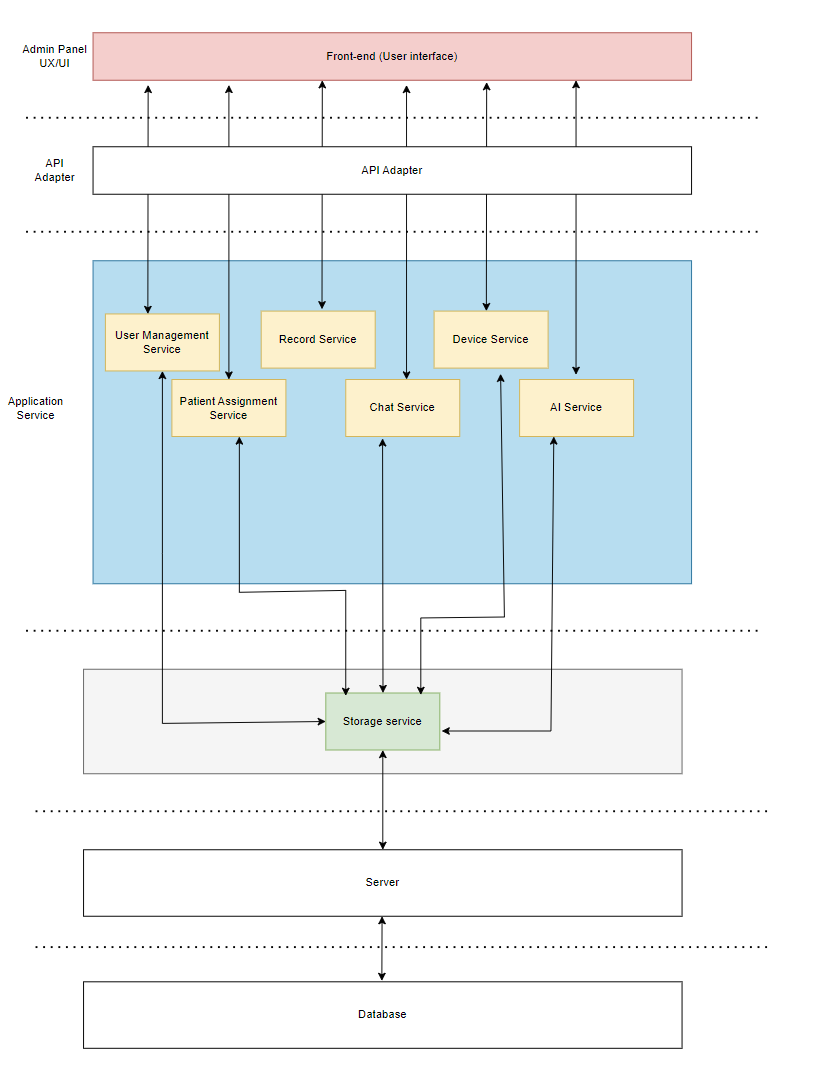
\includegraphics[width=12cm,height=14cm]{Images/system/fmECG_architecture-Admin.drawio.png}
  \caption[Sơ đồ khối cho Website quản trị viên]{\bfseries \fontsize{12pt}{0pt}\selectfont Sơ đồ khối cho Website quản trị viên}
  \label{fmECG_architecture-Admin} %đặt tên cho ảnh
\end{figure}

Quản trị viên sẽ quản lý 2 Services chính đó là quản lý người dùng (User Management Service) và quản lý phân công
bác sĩ - bệnh nhân (Patient Assignment Service), logic và thứ tự các khối tương đồng với ứng dụng dành cho bác sĩ.

Tiếp theo để phân tích cụ thể hơn từng luồng trong hệ thống qua use case, chúng em xin phép được trình bày các sơ đồ tuần
tự. 
\newpage


\subsection{Thiết kế cơ sở dữ liệu}
\label{design_database}


\subsubsection{Chuyển mô hình thực thể liên kết sang mô hình quan hệ}

\begin{itemize}
  \item Người dùng (\textbf{ID người dùng}, Mật khẩu, Email, Tên, Ngày sinh, Số điện thoại, Quyền)
  \item Bản ghi ECG (\textbf{ID bản ghi ECG}, ID người dùng, ID thiết bị, Đường dẫn lưu trữ dữ liệu, Thời gian bắt đầu đo, Thời gian kết thúc đo, Loại cảm biến)
  \item Danh mục tin tức (\textbf{ID danh mục tin tức}, Tên danh mục tin tức, Mô tả danh mục tin tức)
  \item Tin tức (\textbf{ID tin tức}, Tiêu đề, Nội dung, ID danh mục tin tức, Tác giả, Đường dẫn, Đường dẫn hình ảnh)
  \item Phân công bệnh nhân - bác sĩ (\textbf{ID phân công}, ID bệnh nhân, ID bác sĩ, Ngày bắt đầu)
  \item Mã thông báo đặt lại mật khẩu (\textbf{ID mã thông báo}, ID người dùng, Mã thông báo, Thời gian hết hạn)
  \item Phiên đăng nhập (\textbf{ID phiên đăng nhập}, ID người dùng, Mã phiên đăng nhập, Thời gian hết hạn)
  \item Thông tin hội thoại (\textbf{ID hội thoại}, Danh sách ID người dùng trong hội thoại, thông tin tin nhắn gần nhất)
  \item Thông tin tin nhắn (\textbf{ID tin nhắn}, Nội dung tin nhắn, ID người gửi tin nhắn, thời gian gửi tin nhắn, ID hội thoại)
  \item Firebase token người dùng (\textbf{ID token}, Firebase token, ID người dùng)
\end{itemize}


\subsubsection{Chuẩn hoá 3NF}
Các bảng đã được thiết kế theo nguyên tắc chuẩn hoá 3NF, vì không có thuộc tính lặp lại và các thuộc tính không phụ thuộc vào một tập hợp con của khóa chính.

\paragraph{Chuẩn hoá bảng Người dùng}
\mbox{}

\begin{table}[H]
  \caption{\bfseries \fontsize{12pt}{0pt}\selectfont Bảng chuẩn hoá bảng Người dùng}
  \centering
  \begin{tabularx}{0.9\textwidth}{|X|X|}
    \hline
    \textbf{Danh sách thuộc tính} & ID người dùng, Mật khẩu, Email, Tên, Ngày sinh, Số điện thoại,
    Quyền \\ % Thêm \textbf{} cho abc
    \hline
    \textbf{Quy tắc nghiệp vụ} & \textbf{Phụ thuộc hàm} \\
    \hline
    Mỗi người dùng có một ID riêng, có duy nhất mật khẩu, email, tên, ngày sinh, số điện thoại,
    quyền & \parbox[t]{\linewidth}{$\text{ID người dùng} \rightarrow$ mật khẩu, email, tên, ngày sinh, số điện thoại, quyền} \\
    \hline
    \multicolumn{2}{|X|}{$\Rightarrow \text{Khoá chính của bảng: ID người dùng}$} \\
    \multicolumn{2}{|X|}{$\Rightarrow \text{Bảng Người dùng đã ở 3NF}$} \\
    \hline
  \end{tabularx}
\end{table}


\subsubsection{Từ điển dữ liệu}



\begin{table}[H]
  \caption{\bfseries \fontsize{12pt}{0pt}\selectfont Bảng user}
  \centering
  \begin{tabularx}{0.9\textwidth}{|c|c|X|}
    \hline
    \textbf{Thuộc tính} & \textbf{Kiểu dữ liệu} & \textbf{Mô tả} \\
    \hline
    user\_id & INTEGER & Khóa chính của bảng, đại diện cho ID người dùng. \\
    \hline
    password & STRING & Mật khẩu của người dùng. \\
    \hline
    email & STRING & Địa chỉ email của người dùng. \\
    \hline
    name & STRING & Tên của người dùng. \\
    \hline
    doB & DATE & Ngày sinh của người dùng. \\
    \hline
    phone\_number & STRING & Số điện thoại của người dùng. \\
    \hline
    role & INTEGER & Quyền của người dùng (0-patient, 1-doctor, 2-admin). \\
    \hline
    created\_at & DATE & Thời điểm thêm mới dữ liệu vào database. \\
    \hline
    updated\_at & DATE & Thời điểm cập nhật dữ liệu vào database. \\
    \hline
    
  \end{tabularx}
\end{table}

\begin{table}[H]
  \caption{\bfseries \fontsize{12pt}{0pt}\selectfont Bảng ecg\_record}
  \centering
  \begin{tabularx}{0.9\textwidth}{|c|c|X|}
    \hline
    \textbf{Thuộc tính} & \textbf{Kiểu dữ liệu} & \textbf{Mô tả} \\
    \hline
    record\_id & INTEGER & Khóa chính của bảng, đại diện cho ID bản ghi ECG. \\
    \hline
    user\_id & INTEGER & Khóa ngoại tham chiếu đến \texttt{user\_id} trong bảng \texttt{user}. \\
    \hline
    device\_id & STRING & ID thiết bị. \\
    \hline
    data\_directory & STRING & Đường dẫn lưu trữ dữ liệu. \\
    \hline
    start\_time & DATE & Thời gian bắt đầu ghi lại ECG. \\
    \hline
    stop\_time & DATE & Thời gian kết thúc ghi lại ECG. \\
    \hline
    sensor\_type & STRING & Loại cảm biến. \\
    \hline
    created\_at & DATE & Thời điểm thêm mới dữ liệu vào database. \\
    \hline
    updated\_at & DATE & Thời điểm cập nhật dữ liệu vào database. \\
    \hline
  \end{tabularx}
\end{table}

\begin{table}[H]
  \caption{\bfseries \fontsize{12pt}{0pt}\selectfont Bảng news\_category}
  \centering
  \begin{tabularx}{0.9\textwidth}{|c|c|X|}
    \hline
    \textbf{Thuộc tính} & \textbf{Kiểu dữ liệu} & \textbf{Mô tả} \\
    \hline
    category\_id & INTEGER & Khóa chính của bảng, đại diện cho ID danh mục tin tức. \\
    \hline
    category\_name & STRING & Tên danh mục tin tức. \\
    \hline
    category\_description & STRING & Mô tả danh mục tin tức. \\
    \hline
    created\_at & DATE & Thời điểm thêm mới dữ liệu vào database. \\
    \hline
    updated\_at & DATE & Thời điểm cập nhật dữ liệu vào database. \\
    \hline
  \end{tabularx}
\end{table}

\begin{table}[H]
  \caption{\bfseries \fontsize{12pt}{0pt}\selectfont Bảng news}
  \centering
  \begin{tabularx}{0.9\textwidth}{|c|c|X|}
    \hline
    \textbf{Thuộc tính} & \textbf{Kiểu dữ liệu} & \textbf{Mô tả} \\
    \hline
    news\_id & INTEGER & Khóa chính của bảng, đại diện cho ID tin tức. \\
    \hline
    title & STRING & Tiêu đề tin tức. \\
    \hline
    content & TEXT & Nội dung tin tức. \\
    \hline
    category\_id & INTEGER & Khóa ngoại tham chiếu đến \texttt{category\_id} trong bảng \texttt{news\_category}. \\
    \hline
    author & STRING & Tác giả tin tức. \\
    \hline
    url & STRING & Đường dẫn tin tức. \\
    \hline
    image & STRING & Đường dẫn hình ảnh tin tức (có thể là null). \\
    \hline
    created\_at & DATE & Thời điểm thêm mới dữ liệu vào database. \\
    \hline
    updated\_at & DATE & Thời điểm cập nhật dữ liệu vào database. \\
    \hline
  \end{tabularx}
\end{table}

\begin{table}[H]
  \caption{\bfseries \fontsize{12pt}{0pt}\selectfont Bảng patient\_doctor\_assignment}
  \centering
  \begin{tabularx}{0.9\textwidth}{|c|c|X|}
    \hline
    \textbf{Thuộc tính} & \textbf{Kiểu dữ liệu} & \textbf{Mô tả} \\
    \hline
    assign\_id & INTEGER & Khóa chính của bảng, đại diện cho ID phân công bệnh nhân - bác sĩ. \\
    \hline
    patient\_id & INTEGER & Khóa ngoại tham chiếu đến \texttt{user\_id} trong bảng \texttt{user} (với quyền là bệnh nhân). \\
    \hline
    doctor\_id & INTEGER & Khóa ngoại tham chiếu đến \texttt{user\_id} trong bảng \texttt{user} (với quyền là bác sĩ). \\
    \hline
    start\_date & DATE & Ngày bắt đầu phân công. \\
    \hline
    created\_at & DATE & Thời điểm thêm mới dữ liệu vào database. \\
    \hline
    updated\_at & DATE & Thời điểm cập nhật dữ liệu vào database. \\
    \hline
  \end{tabularx}
\end{table}

\begin{table}[H]
  \caption{\bfseries \fontsize{12pt}{0pt}\selectfont Bảng reset\_token}
  \centering
  \begin{tabularx}{0.9\textwidth}{|c|c|X|}
    \hline
    \textbf{Thuộc tính} & \textbf{Kiểu dữ liệu} & \textbf{Mô tả} \\
    \hline
    id & INTEGER & Khóa chính của bảng, đại diện cho ID mã thông báo đặt lại. \\
    \hline
    user\_id & INTEGER & Khóa ngoại tham chiếu đến \texttt{user\_id} trong bảng \texttt{user}. \\
    \hline
    token & STRING & Mã thông báo đặt lại. \\
    \hline
    expiration & DATE & Thời gian hết hạn của mã thông báo đặt lại. \\
    \hline
    created\_at & DATE & Thời điểm thêm mới dữ liệu vào database. \\
    \hline
    updated\_at & DATE & Thời điểm cập nhật dữ liệu vào database. \\
    \hline
  \end{tabularx}
\end{table}


\begin{table}[H]
  \caption{\bfseries \fontsize{12pt}{0pt}\selectfont Bảng session}
  \centering
  \begin{tabularx}{0.9\textwidth}{|c|c|X|}
    \hline
    \textbf{Thuộc tính} & \textbf{Kiểu dữ liệu} & \textbf{Mô tả} \\
    \hline
    session\_id & INTEGER & Khóa chính của bảng, đại diện cho ID phiên đăng nhập. \\
    \hline
    user\_id & INTEGER & Khóa ngoại tham chiếu đến \texttt{user\_id} trong bảng \texttt{user}. \\
    \hline
    token & STRING & Mã phiên đăng nhập. \\
    \hline
    expiration & DATE & Thời gian hết hạn của phiên đăng nhập. \\
    \hline
    created\_at & DATE & Thời điểm thêm mới dữ liệu vào database. \\
    \hline
    updated\_at & DATE & Thời điểm cập nhật dữ liệu vào database. \\
    \hline
  \end{tabularx}
\end{table}

\begin{table}[H]
  \caption{\bfseries \fontsize{12pt}{0pt}\selectfont Bảng device}
  \centering
  \begin{tabularx}{0.9\textwidth}{|c|c|X|}
    \hline
    \textbf{Thuộc tính} & \textbf{Kiểu dữ liệu} & \textbf{Mô tả} \\
    \hline
    device\_id & INTEGER & Khóa chính của bảng, đại diện cho ID thiết bị. \\
    \hline
    device\_name & STRING & Tên thiết bị. \\
    \hline
    created\_at & DATE & Thời điểm thêm mới dữ liệu vào database. \\
    \hline
    updated\_at & DATE & Thời điểm cập nhật dữ liệu vào database. \\
    \hline
  \end{tabularx}
\end{table}

\begin{table}[H]
  \caption{\bfseries \fontsize{12pt}{0pt}\selectfont Bảng conversation}
  \centering
  \begin{tabularx}{0.9\textwidth}{|c|c|X|}
    \hline
    \textbf{Thuộc tính} & \textbf{Kiểu dữ liệu} & \textbf{Mô tả} \\
    \hline
    conversation\_id & STRING & Khóa chính của bảng, đại diện cho ID hội thoại \\
    \hline
    members\_id & MAP<String, Boolean> & Danh sách ID của người dùng trong hội thoại \\
    \hline
    recent\_message & MAP<String, dynamic> & Thông tin tin nhắn gần nhất \\
    \hline
    created\_at & DATE & Thời điểm thêm mới dữ liệu vào database \\
    \hline
    updated\_at & DATE & Thời điểm cập nhật dữ liệu vào database \\
    \hline
  \end{tabularx}
\end{table}

\begin{table}[H]
  \caption{\bfseries \fontsize{12pt}{0pt}\selectfont Bảng message}
  \centering
  \begin{tabularx}{0.9\textwidth}{|c|c|X|}
    \hline
    \textbf{Thuộc tính} & \textbf{Kiểu dữ liệu} & \textbf{Mô tả} \\
    \hline
    message\_id & STRING & Khóa chính của bảng, đại diện cho ID tin nhắn \\
    \hline
    conversation\_id & STRING & ID hội thoại chứa tin nhắn \\
    \hline
    message\_content & STRING & Nội dung tin nhắn \\
    \hline
    sender\_id & INTEGER & ID Người gửi tin nhắn\\
    \hline
    created\_at & DATE & Thời điểm thêm mới dữ liệu vào database \\
    \hline
    updated\_at & DATE & Thời điểm cập nhật dữ liệu vào database \\
    \hline
  \end{tabularx}
\end{table}

\begin{table}[H]
  \caption{\bfseries \fontsize{12pt}{0pt}\selectfont Bảng user\_firebase\_token}
  \centering
  \begin{tabularx}{0.9\textwidth}{|c|c|X|}
    \hline
    \textbf{Thuộc tính} & \textbf{Kiểu dữ liệu} & \textbf{Mô tả} \\
    \hline
    token\_id & String & Khóa chính của bảng, đại diện cho ID firebase token \\
    \hline
    firebase\_token & STRING & Token của thiết bị đăng nhập vào hệ thống do Firebase sinh ra \\
    \hline
    user\_id & INTEGER & ID của người dùng sử dụng token \\
    \hline
    created\_at & DATE & Thời điểm thêm mới dữ liệu vào database. \\
    \hline
    updated\_at & DATE & Thời điểm cập nhật dữ liệu vào database. \\
    \hline
  \end{tabularx}
\end{table}

\subsubsection{Sơ đồ ERD}

\begin{figure}[H]
  \centering
  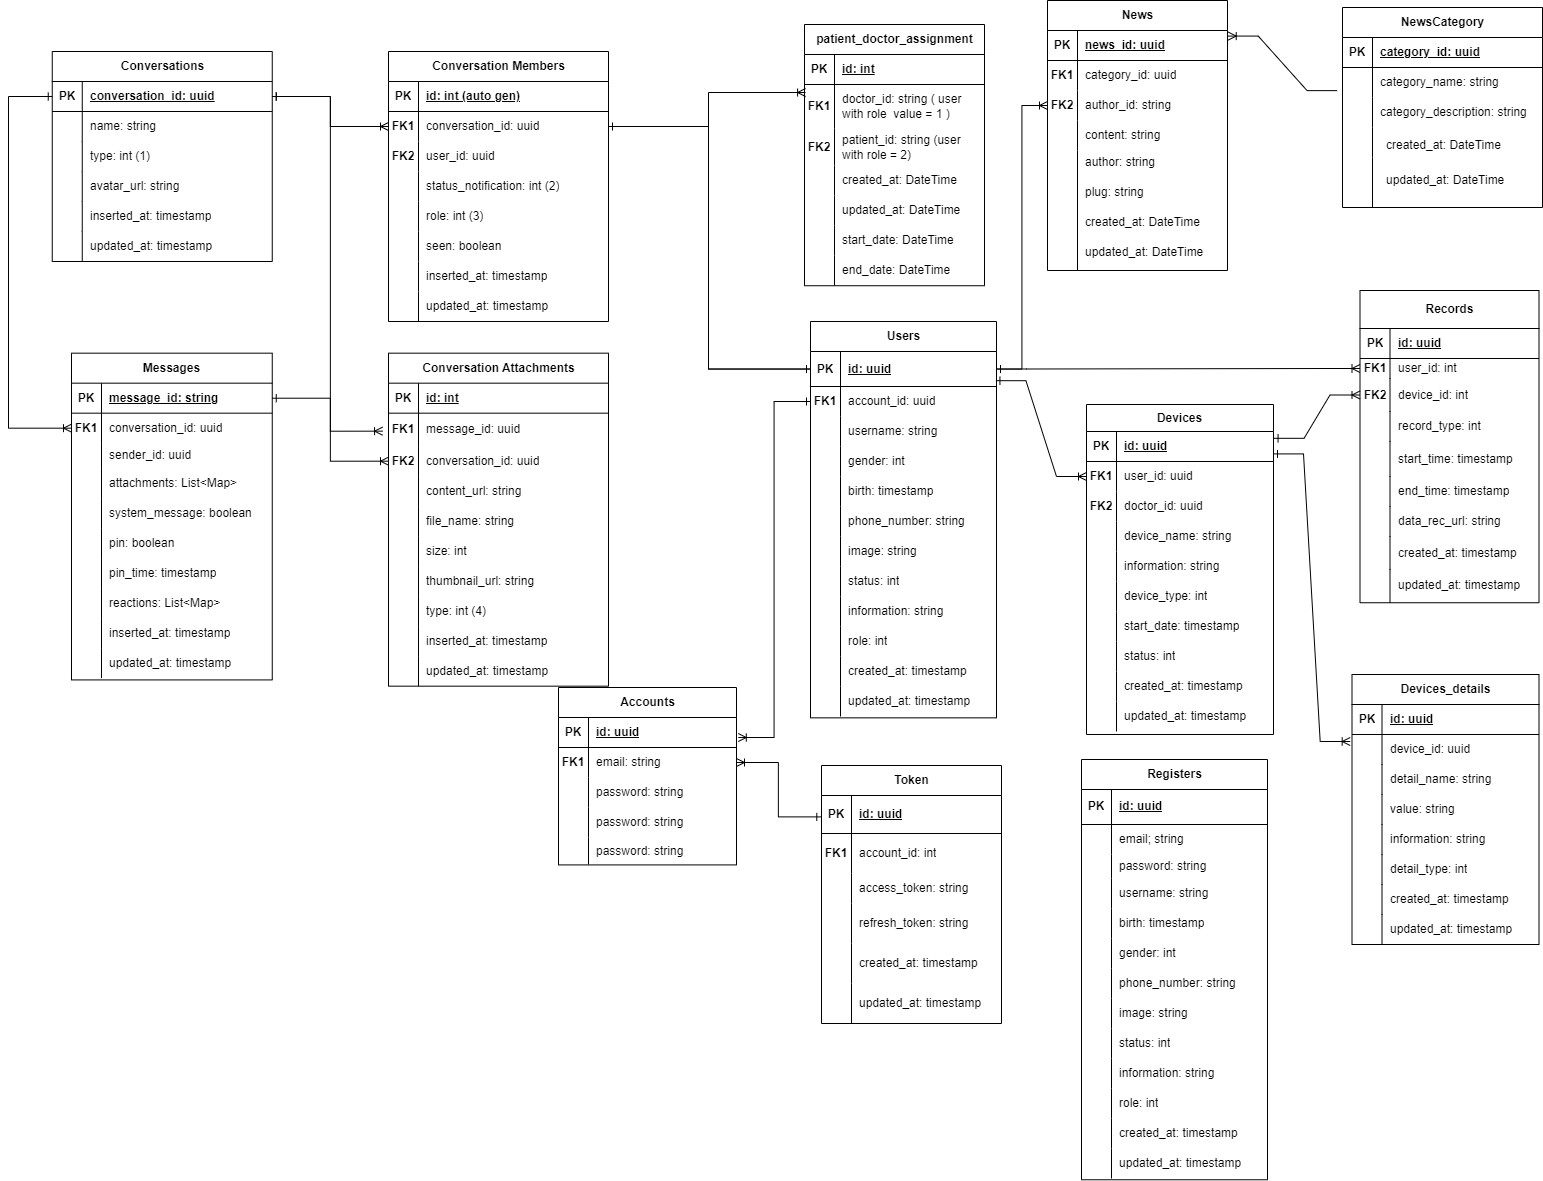
\includegraphics[width=15cm,height=15cm]{Images/system/fmECG_database.png}
  \caption[Sơ đồ ERD]{\bfseries \fontsize{12pt}{0pt}\selectfont Sơ đồ ERD}
  \label{fmECG_architecture-Database} %đặt tên cho ảnh
\end{figure}

\subsection{Thiết kế giao diện}

\subsubsection{Website}

Dưới đây là các giao diện thực tế mà chúng em thiết kế cho trang web quản trị


\begin{figure}[H]
  \centering
  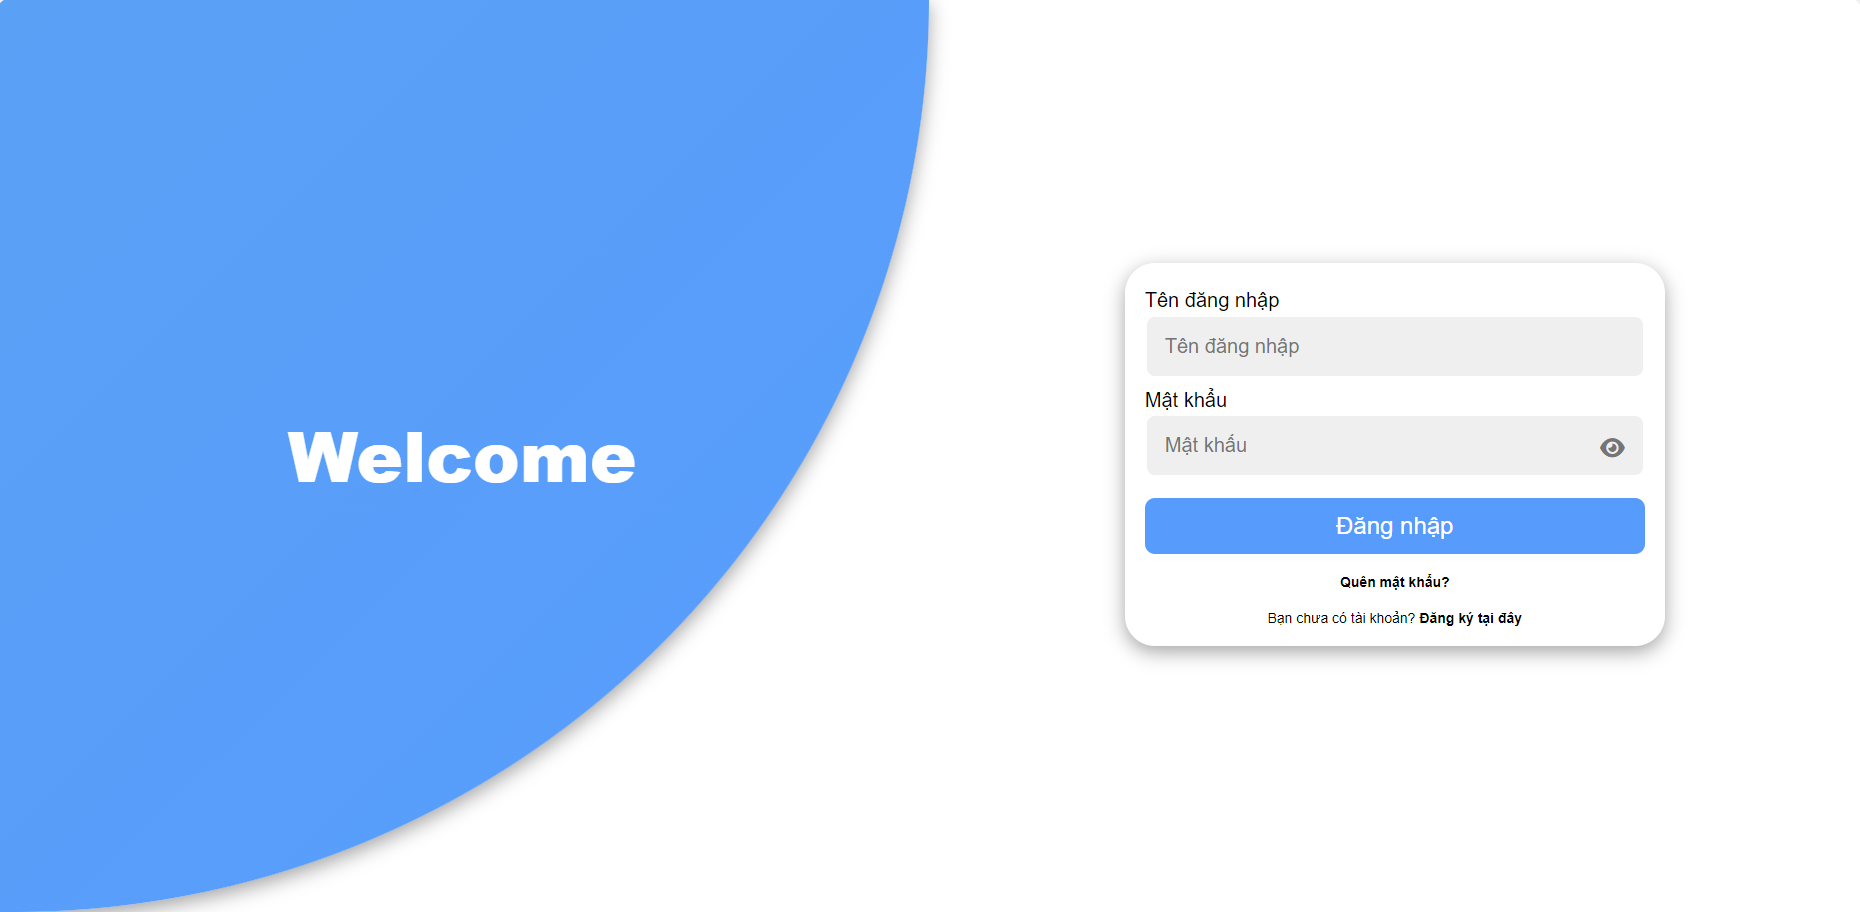
\includegraphics[scale=0.7]{Images/server/webUI/login.PNG}
  \caption[Giao diện trang đăng nhập]{\bfseries \fontsize{12pt}{0pt}\selectfont Giao diện trang đăng nhập}
  \label{login} %đặt tên cho ảnh
\end{figure}

Hình \ref{login} mô tả giao diện cho màn hình đăng nhập, màn hình này sẽ bao
 gồm hai trường thông tin là Email và Password để admin đăng nhập vào trang quản trị
 nếu hai trường thông tin email và password là chính xác thì sẽ chuyển hướng đến trang dashboard 
 quản lý như hình \ref{dashboard}, còn nếu sai thông tin thì sẽ có popup thông báo sai email hoặc mật khẩu hiện lên
 

\subsection{Sơ đồ lớp cho ứng dụng di động, website và server}

\subsubsection{Server và Website quản trị hệ thống}


\begin{enumerate}[a)]
\item Danh sách các class diagram

\begin{figure}[H]
  \centering
  \includegraphics[width=16cm,height=13cm]{Images/server/class/class_controller.png}
  \caption[Sơ đồ lớp của package Controllers]{\bfseries \fontsize{12pt}{0pt}\selectfont Sơ đồ lớp của package Controllers}
  \label{class_controller} %đặt tên cho ảnh
\end{figure}



\begin{figure}[H]
  \centering
  \includegraphics[width=15cm,height=16cm]{Images/server/class/class_model.png}
  \caption[Sơ đồ lớp của package Models]{\bfseries \fontsize{12pt}{0pt}\selectfont Sơ đồ lớp của package Models}
  \label{class_model} %đặt tên cho ảnh
\end{figure}


\begin{figure}[H]
  \centering
  \includegraphics[width=14cm,height=6cm]{Images/server/class/class_route.png}
  \caption[Sơ đồ lớp của package Routes]{\bfseries \fontsize{12pt}{0pt}\selectfont Sơ đồ lớp của package Routes}
  \label{class_route} %đặt tên cho ảnh
\end{figure}


\begin{figure}[H]
  \centering
  \includegraphics[width=15cm,height=14cm]{Images/server/class/class_admin.png}
  \caption[Sơ đồ lớp của package View và Admin]{\bfseries \fontsize{12pt}{0pt}\selectfont Sơ đồ lớp của package View và Admin}
  \label{class_admin} %đặt tên cho ảnh
\end{figure}


\begin{itemize}

  \item Package "Controllers":

  Chứa các controllers xử lý logic và điều khiển các yêu cầu từ người dùng.
  \item Package "Models":
  
  Chứa các lớp đại diện cho các đối tượng của cơ sở dữ liệu, định nghĩa các thuộc tính và phương thức để làm việc với dữ liệu.
  \item Package "Routes":
  
  Chứa các lớp route, xác định các endpoint và xử lý các yêu cầu HTTP từ người dùng bằng cách gọi tới các controllers tương ứng.
  \item Package "Views":
  
  Chứa các view components đại diện cho giao diện người dùng.
  \item Package "Admin":
  
  Chứa các thành phần liên quan đến trang Admin dashboard.
  \item Package "Resources" (Trong "Admin"):
  
  Chứa các lớp Resource (nguồn tài nguyên) đại diện cho các tài nguyên của trang Admin dashboard, bao gồm: AdminResource, DoctorResource, PatientResource, ECGRecordResource, NewsResource, NewsCategoryResource và PatientDoctorAssignmentResource.
  \item Package "Components" (Trong "Admin"):
  
  Chứa các lớp Components đại diện cho các thành phần giao diện của trang Admin dashboard, bao gồm: ComponentLoader, DashboardViewComponent, NewsViewComponent, ECGRecordViewComponent và PatientDoctorAssignmentViewComponent.
\end{itemize}



\item Mối quan hệ

\begin{figure}[H]
  \centering
  \includegraphics[width=15cm,height=12cm]{Images/server/class/class_relation.png}
  \caption[Mối quan hệ giữa các class ở phía server]{\bfseries \fontsize{12pt}{0pt}\selectfont Mối quan hệ giữa các class ở phía server}
  \label{class_relation} %đặt tên cho ảnh
\end{figure}
Hình \ref{class_relation} mô tả mối quan hệ giữa các class ở phía server để cung cấp API 
Các class ở package Controllers sử dụng  đối tượng của các class ở package Models. 
Và tương tự các class ở package Routes cũng sử dụng  đối tượng của các class ở package Controllers.
 
\begin{figure}[H]
  \centering
  \includegraphics[width=16cm,height=15cm]{Images/server/class/class_admin_relation.png}
  \caption[Mối quan hệ giữa các class ở phía website quản trị]{\bfseries \fontsize{12pt}{0pt}\selectfont Mối quan hệ giữa các class ở phía website quản trị}
  \label{class_admin_relation} %đặt tên cho ảnh
\end{figure}
Hình \ref{class_admin_relation} mô tả mối quan hệ giữa các class ở phía website quản trị. 
Các class ở package Resources sử dụng  đối tượng của các class ở package Models. 
Class ở package Components sử dụng  đối tượng của các class ở package Views. 
Rồi class AdminController ở package Controllers sử dụng  đối tượng của các class ở package Resources và Components. 
Và class AdminRoute ở package Routes sử dụng  đối tượng của class AdminController
\end{enumerate}



\subsection{Thiết kế các chức năng cho website và server}

\subsubsection{Thiết kế API}


\begin{enumerate}[a)]
  \item API liên quan đến thông tin người dùng
  

  \begin{table}[H]
    \centering
    \caption{\bfseries \fontsize{12pt}{0pt}\selectfont Bảng API liên quan đến thông tin người dùng}
    \begin{tabularx}{0.9\textwidth}{
    | >{\raggedright\arraybackslash}X
    | >{\raggedright\arraybackslash}m{2cm}
    | >{\raggedright\arraybackslash}X|
    }
    \hline
    \bfseries Đường dẫn    &\bfseries Phương thức    &\bfseries Mô tả\\ \hline
   api/users/profile   &   GET  &  Lấy thông tin của người dùng với đầu vào là JWT token khi người dùng đăng nhập thành công vào hệ thống \\  \hline
   api/users/profile   &    PUT    &  Cập nhật thông tin người dùng \\  \hline
   api/users/change-password   &   PUT     & Thay đổi mật khẩu của người dùng  \\ \hline
   api/users/\{:userId\}  &   GET     & Lấy thông tin của người dùng cụ thể theo user id \\ \hline

    \end{tabularx}
    \label{table_api_user}
\end{table}

\item API liên quan đến việc xác thực người dùng


\begin{table}[H]
  \centering
  \caption{\bfseries \fontsize{12pt}{0pt}\selectfont Bảng API liên quan đến việc xác thực người dùng}
  \begin{tabularx}{0.9\textwidth}{
  | >{\raggedright\arraybackslash}X
  | >{\raggedright\arraybackslash}m{2cm}
  | >{\raggedright\arraybackslash}X|
  }
  \hline
  \bfseries Đường dẫn    &\bfseries Phương thức    &\bfseries Mô tả\\ \hline
 api/register   &   POST  & Đăng ký tài khoản \\ \hline
 api/login   &    POST    & Đăng nhập vào hệ thống \\ \hline
 api/logout  &   GET     & Đăng xuất khỏi hệ thống \\ \hline
 api/reset-password  &     POST   &  Gửi reset token đến email của người dùng để reset mật khẩu \\  \hline
 api/reset-password/reset &   POST     & Giúp reset lại mật khẩu mới với verify token được nhận từ api: api/reset-password  \\ \hline

  \end{tabularx}
  \label{table_api_auth}
\end{table}


\item API liên quan đến tin tức


\begin{table}[H]
  \centering
  \caption{\bfseries \fontsize{12pt}{0pt}\selectfont Bảng API liên quan đến tin tức}
  \begin{tabularx}{0.9\textwidth}{
  | >{\raggedright\arraybackslash}X
  | >{\raggedright\arraybackslash}m{2cm}
  | >{\raggedright\arraybackslash}X|
  }
  \hline
  \bfseries Đường dẫn    &\bfseries Phương thức    &\bfseries Mô tả\\ \hline
 api/news/\{:newsId\}   &   GET  & Lấy nội của tin tức tương ứng với id dưới dạng HTML \\ \hline
 api/news   &    GET    & Lấy toàn bộ danh sách thông tin của tin tức \\ \hline
 api/categories  &   GET     & Lấy toàn bộ danh sách thông tin của tin tức \\ \hline
 api/category/\{:categoryId\}   &     GET   & Lấy thông tin của loại tin tức theo id tương ứng \\ \hline
 api/ news/category/\{:categoryId\} &   GET     & Lấy toàn bộ thông tin của tin tức theo id của loại tin \\ \hline

  \end{tabularx}
  \label{table_api_news}
\end{table}

\item API liên quan đến bản ghi ECG


\begin{table}[H]
  \centering
  \caption{\bfseries \fontsize{12pt}{0pt}\selectfont Bảng API liên quan đến bản ghi ECG}
  \begin{tabularx}{0.9\textwidth}{
  | >{\raggedright\arraybackslash}X
  | >{\raggedright\arraybackslash}m{2cm}
  | >{\raggedright\arraybackslash}X|
  }
  \hline
  \bfseries Đường dẫn    &\bfseries Phương thức    &\bfseries Mô tả\\ \hline
 api/ecg-records/upload   &   POST  & Tải dữ liệu của phiên đo ECG lên server \\ \hline
 api/ecg-records/patient/\{:patientId\}   &    GET    & Lấy danh sách thông tin các phiên đo ECG của bệnh nhân \\ \hline
 api/ecg-records/doctor/\{:doctorId\} &   GET     & Lấy danh sách thông tin các phiên đo ECG của các bệnh nhân được quản lý bởi bác sỹ \\ \hline
 api/ecg-records/record-data/\{:recordId\}  &     GET   & Lấy dữ liệu một phiên đo của bệnh nhân \\ \hline

  \end{tabularx}
  \label{table_api_ecg}
\end{table}


\item API liên quan liên quan đến việc phân công bệnh nhân cho bác sỹ



\begin{table}[H]
  \centering
  \caption{\bfseries \fontsize{12pt}{0pt}\selectfont Bảng API liên quan liên quan đến việc phân công bệnh nhân cho bác sỹ}
  \begin{tabularx}{0.9\textwidth}{
  | >{\raggedright\arraybackslash}X
  | >{\raggedright\arraybackslash}m{2cm}
  | >{\raggedright\arraybackslash}X|
  }
  \hline
  \bfseries Đường dẫn    &\bfseries Phương thức    &\bfseries Mô tả\\ \hline
   api/doctor/\{:doctorId\}/patients   &   GET  & Lấy danh sách thông tin bệnh nhân được phân công cho bác sĩ \\ \hline
  api/patient/\{:patientId\}/doctor  &    GET    & Lấy thông tin bác sỹ được phân công cho bệnh nhân \\ \hline

  \end{tabularx}
  \label{table_api_pat_doc}
\end{table}



\end{enumerate}




\subsubsection{Sơ đồ tuần tự}


% ------------------------User----------------------


\paragraph{API liên quan đến thông tin người dùng}
\mbox{}

% sửa lại ảnh 
\begin{figure}[H]
  \centering
  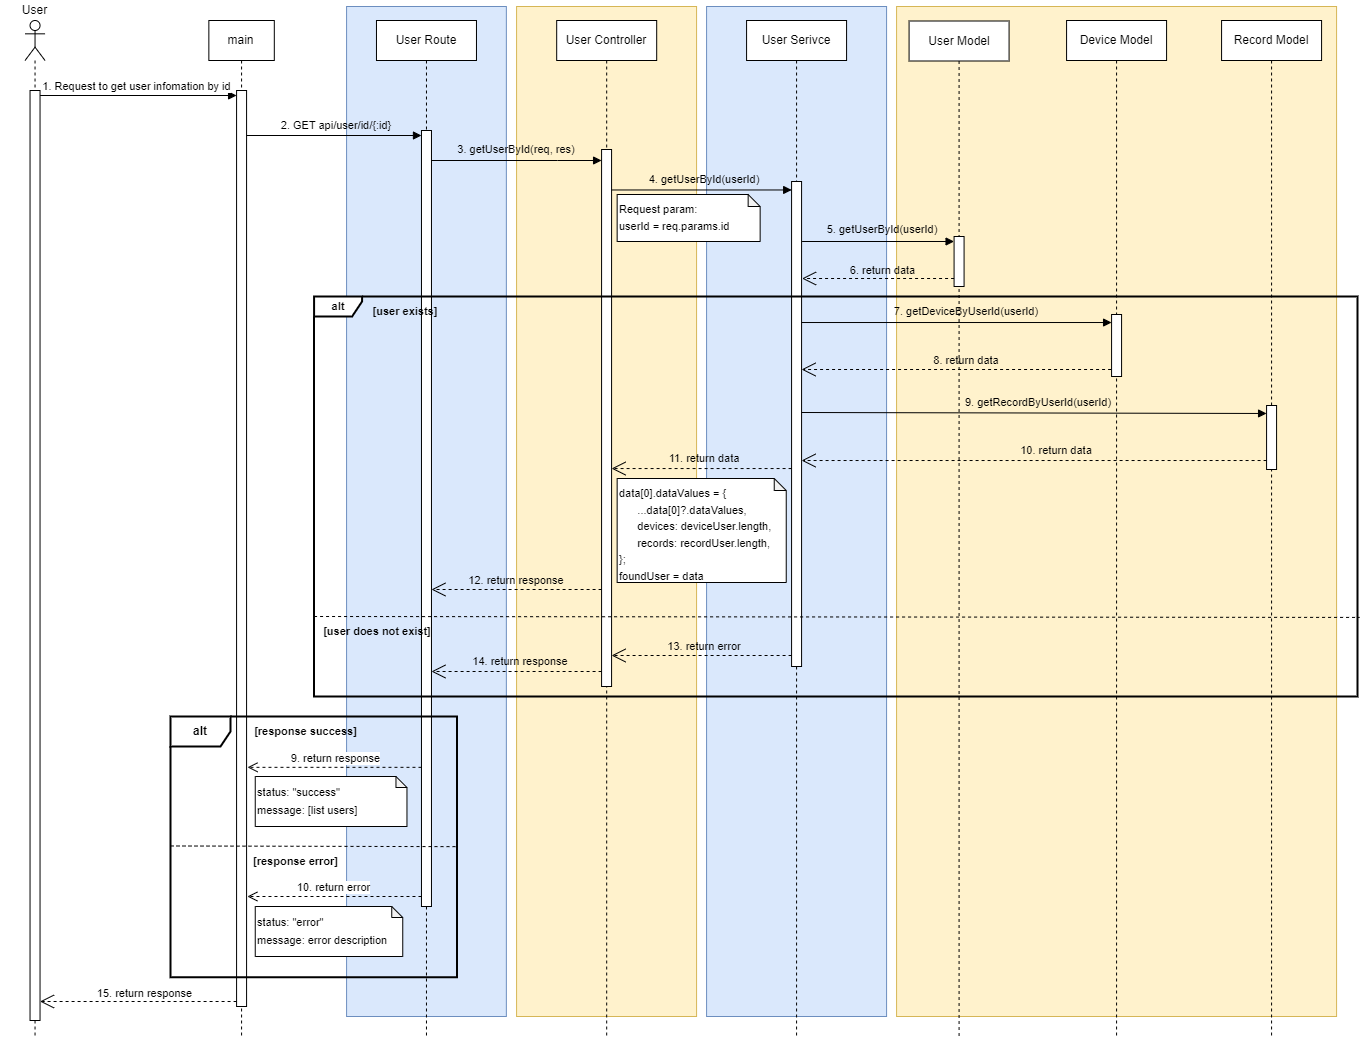
\includegraphics[width=16cm,height=9cm]{Images/server/sequence/server/getUserById.png}
  \caption[Sơ đồ tuần tự cho API lấy thông tin của người dùng dựa trên ID ]{\bfseries \fontsize{12pt}{0pt}
  \selectfont Sơ đồ tuần tự cho API lấy thông tin của người dùng dựa trên ID }
  \label{getUserById} %đặt tên cho ảnh
\end{figure}
Hình \ref{getUserById} mô tả quá trình lấy thông tin người dùng dựa trên ID trong ứng dụng. Người dùng gửi yêu cầu lấy thông tin người dùng theo ID, thông qua các tầng của hệ thống, yêu cầu này được xử lý bởi UserController. UserController kiểm tra thông tin và truy vấn UserModel để lấy thông tin người dùng. Nếu người dùng không tồn tại, hệ thống trả về response lỗi, ngược lại, response chứa thông tin người dùng được gửi lại từ UserController tới người dùng.


% \linebreak


% ----------------------------------------------



% ------------------------Auth----------------------


\paragraph{API liên quan đến việc xác thực người dùng}
\mbox{}

\begin{figure}[H]
  \centering
  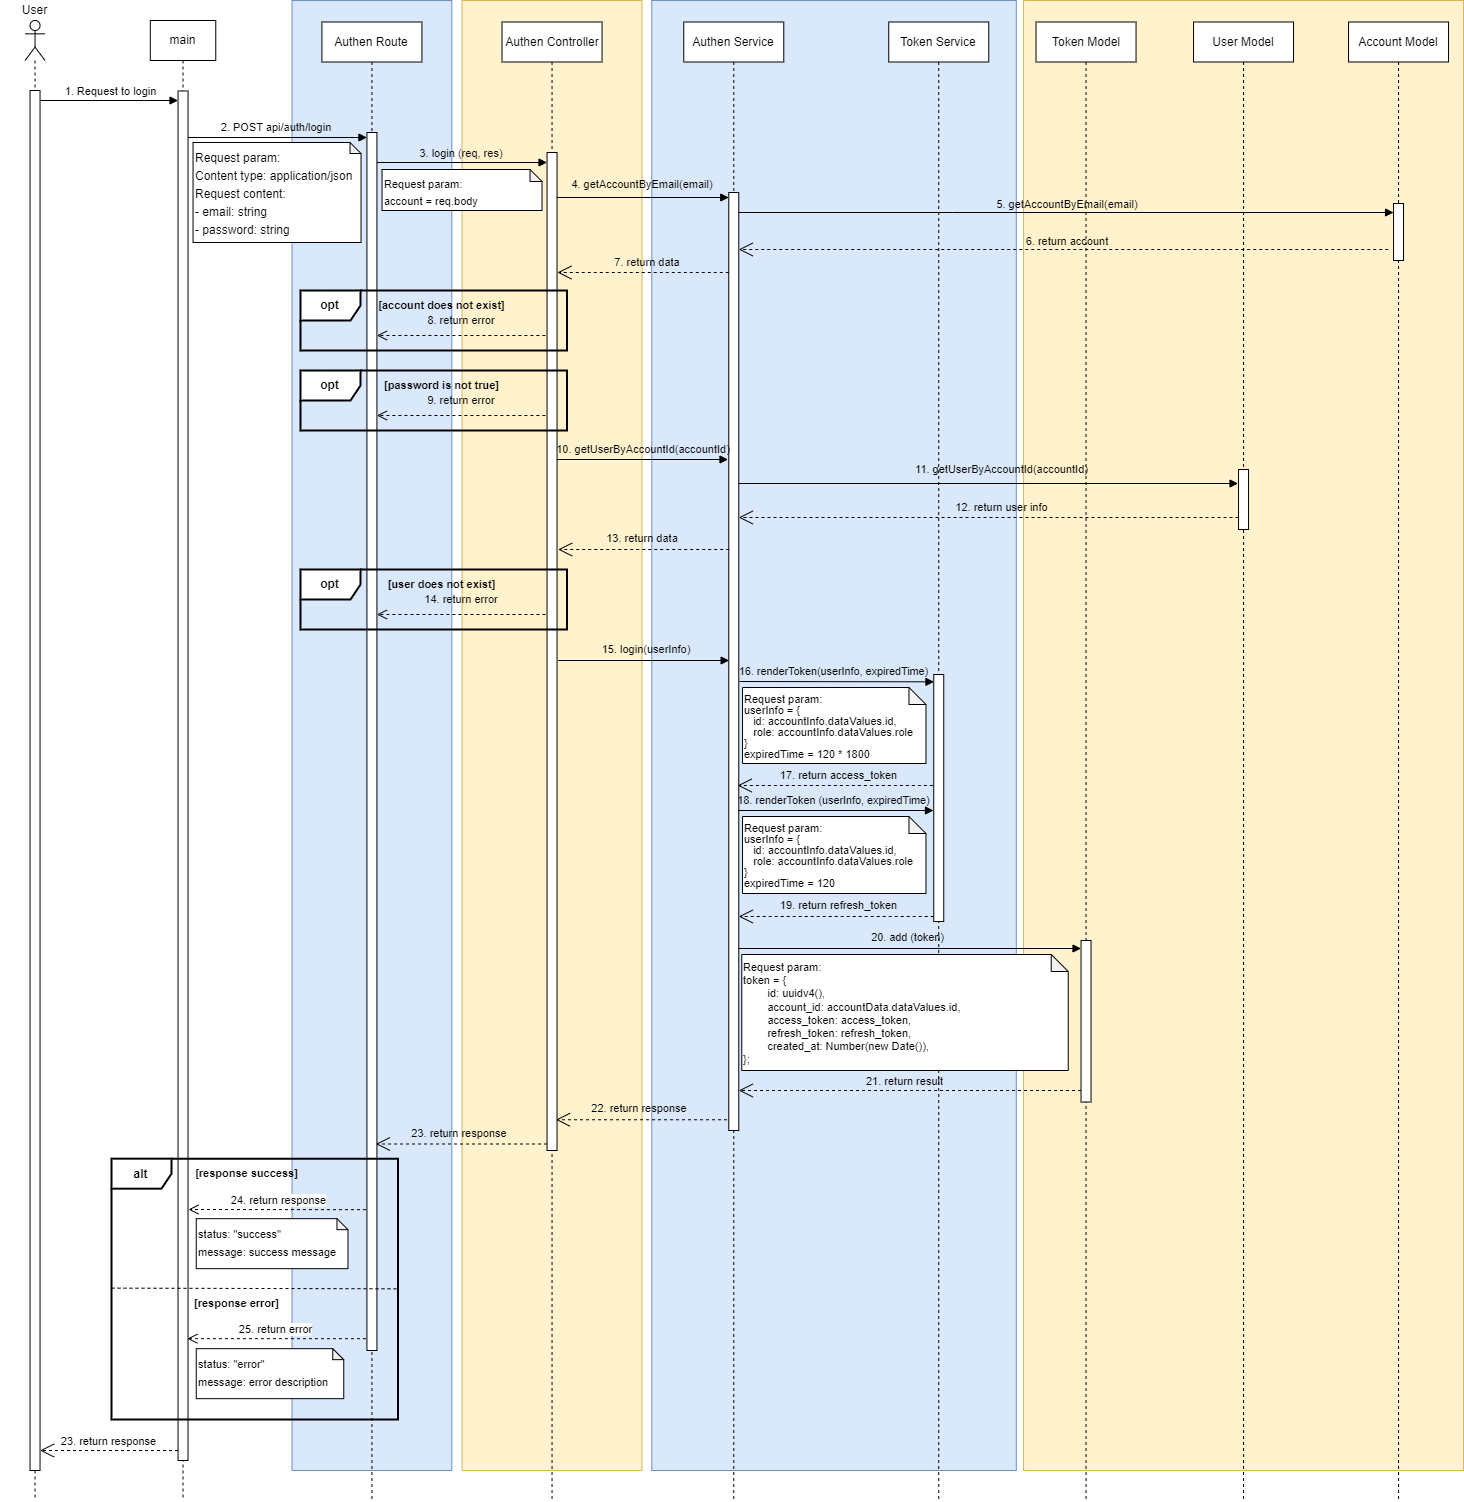
\includegraphics[width=16cm,height=12cm]{Images/server/sequence/server/login.png}
  \caption[Sơ đồ tuần tự cho API đăng nhập vào hệ thống]{\bfseries \fontsize{12pt}{0pt}
  \selectfont Sơ đồ tuần tự cho API đăng nhập vào hệ thống }
  \label{backend_login} %đặt tên cho ảnh
\end{figure}
Hình \ref{backend_login}  mô tả quá trình xác thực người dùng đăng nhập vào ứng dụng. Người dùng gửi yêu cầu đăng nhập, thông qua các tầng của hệ thống, yêu cầu này được xử lý bởi AuthController. AuthController kiểm tra thông tin người dùng, tạo token nếu đúng thông tin đăng nhập và trả về response cho người dùng.

% ----------------------------------------------

% -------------------------ECG----------------------------
\paragraph{API liên quan đến bản ghi ECG}
\mbox{}

\begin{figure}[H]
  \centering
  \includegraphics[width=16cm,height=9cm]{Images/server/sequence/server/getEcgRecordsByDoctor.png}
  \caption[Sơ đồ tuần tự cho API lấy thông tin phiên đo ECG của các bệnh nhân được quản lý bởi một bác sĩ ]{\bfseries \fontsize{12pt}{0pt}
  \selectfont Sơ đồ tuần tự cho API lấy thông tin phiên đo ECG của các bệnh nhân được quản lý bởi một bác sĩ }
  \label{getEcgRecordsByDoctor} %đặt tên cho ảnh
\end{figure}
Hình \ref{getEcgRecordsByDoctor} mô tả quá trình lấy dữ liệu ECG (Electrocardiogram) của tất cả bệnh nhân được quản lý bởi một bác sĩ trong ứng dụng. Người dùng (bác sĩ) gửi yêu cầu lấy dữ liệu ECG của tất cả bệnh nhân mà họ quản lý, thông qua các tầng của hệ thống, yêu cầu này được xử lý bởi ECGRecordController. ECGRecordController tiếp tục truy vấn ECGRecordModel để lấy dữ liệu ECG dựa trên doctorId (ID của bác sĩ) được truyền vào từ yêu cầu. Sau đó, danh sách dữ liệu ECG của các bệnh nhân được trả về từ ECGRecordModel và được gửi trở lại ECGRecordRoute để trả về response cho người dùng. Nếu quá trình thực hiện thành công, hệ thống trả về response chứa danh sách dữ liệu ECG cho bác sĩ. Nếu có lỗi xảy ra trong quá trình này, hệ thống trả về response lỗi tương ứng. Sau khi xử lý, response cuối cùng được trả về tới người dùng (bác sĩ).


% -----------------------------------------------------



% -----------------------PatientDoctor------------------------------

\paragraph{API liên quan liên quan đến việc phân công bệnh nhân cho bác sỹ}
\mbox{}


\begin{figure}[H]
  \centering
  \includegraphics[width=16cm,height=10cm]{Images/server/sequence/server/getDoctorByPatient.png}
  \caption[Sơ đồ tuần tự cho API lấy thông tin bác sĩ được phân công cho một bệnh nhân ]{\bfseries \fontsize{12pt}{0pt}
  \selectfont Sơ đồ tuần tự cho API lấy thông tin bác sĩ được phân công cho một bệnh nhân }
  \label{getDoctorByPatient} %đặt tên cho ảnh
\end{figure}
Hình \ref{getDoctorByPatient} mô tả quá trình lấy thông tin bác sĩ được phân công cho một bệnh nhân cụ thể. Người dùng (User) gửi yêu cầu lấy thông tin bác sĩ của một bệnh nhân cụ thể, thông qua các tầng của hệ thống, yêu cầu này được xử lý bởi PatientDoctorAssignmentController. PatientDoctorAssignmentController tìm kiếm thông tin liên kết giữa bệnh nhân và bác sĩ trong PatientDoctorAssignmentModel bằng cách tìm bản ghi với patient\_id trùng khớp với bệnh nhân được chỉ định. Nếu không tìm thấy thông tin liên kết, hệ thống trả về response lỗi tương ứng. Nếu tìm thấy thông tin liên kết, PatientDoctorAssignmentController sẽ tiếp tục tìm kiếm thông tin của bác sĩ trong UserModel bằng cách sử dụng doctor\_id lấy từ bản ghi liên kết. Sau khi tìm thấy thông tin của bác sĩ, hệ thống trả về response thành công chứa thông tin về bác sĩ đó. Nếu có lỗi xảy ra trong quá trình này, hệ thống trả về response lỗi tương ứng. Sau khi xử lý, response cuối cùng được trả về tới người dùng.

% -----------------------------------------------------

\paragraph{Website quản trị}
\mbox{}


\begin{figure}[H]
  \centering
  \includegraphics[width=16cm,height=10cm]{Images/server/sequence/web/seq_auth.png}
  \caption[Sơ đồ tuần tự cho quá trình truy cập vào trang quản trị (admin dashboard) ]{\bfseries \fontsize{12pt}{0pt}
  \selectfont Sơ đồ tuần tự cho quá trình truy cập vào trang quản trị (admin dashboard) }
  \label{seq_auth} %đặt tên cho ảnh
\end{figure}
Hình \ref{seq_auth} mô tả quá trình truy cập vào bảng điều khiển quản trị (admin dashboard) của người dùng (User). Khi người dùng yêu cầu truy cập vào admin dashboard, hệ thống sẽ yêu cầu xác thực thông qua ViewComponent. Nếu xác thực thành công, AdminJS sẽ xây dựng admin dashboard và yêu cầu dữ liệu từ các tài nguyên (resources) khác nhau để hiển thị thông tin.



Nếu xác thực thành công, AdminJS sẽ yêu cầu dữ liệu từ các tài nguyên khác nhau, bao gồm DoctorResource, AdminResource, PatientResource, NewsResource, NewsCategoryResource, EcgRecordsResource và PatientDoctorAssignmentResource. Mỗi tài nguyên sẽ trả về dữ liệu tương ứng và AdminJS sẽ sử dụng các dữ liệu này để hiển thị trên admin dashboard.



Sau khi AdminJS đã thu thập đủ dữ liệu từ các tài nguyên, nó sẽ chuyển hướng ViewComponent đến trang /admin để hiển thị admin dashboard cho người dùng. Nếu xác thực không thành công, AdminJS sẽ chuyển hướng ViewComponent đến trang /admin/login để hiển thị trang đăng nhập cho người dùng.



Sau khi hoàn tất, hệ thống sẽ trả về response cuối cùng và hiển thị trang tương ứng cho người dùng.


\subsection{Thiết kế các chức năng cho ứng dụng di động}
\label{design_function_mobile}

Ứng dụng di động được trong hệ thống được chia cụ thể gồm ứng dụng di động cho bệnh nhân và ứng dụng di động cho bác sĩ. 
Hầu hết các chức năng cơ bản được thể hiện trong sơ đồ usecase của hai ứng dụng đều giống nhau như đăng nhập, xem lịch sử đo, nhắn tin.
Điểm khác biệt giữa hai ứng dụng di động là ứng dụng di động cho bệnh nhân sẽ có thêm chức năng kết nối với thiết bị đo cũng như xem tin tức.

Trong nội dung của mục \ref{design_function_mobile}, chúng em xin được phép trình bày chi tiết hướng thực hiện các chức năng
từ các chức năng chung đến chức năng riêng cho bệnh nhân, đồng thời sẽ triển khai hướng tối ưu của từng chức năng (nếu có).

Các chức năng chung của hai ứng dụng cho bác sĩ và bệnh nhân bao gồm: 

\begin{adjustwidth}{1.5em}{}
\begin{itemize}
  \item Chức năng đăng nhập
  \item Chức năng xem lịch sử đo
  \item Chức năng nhắn tin.
\end{itemize}
\end{adjustwidth}

Các chức năng riêng của bệnh nhân bao gồm:
\begin{adjustwidth}{1.5em}{}
\begin{itemize}
  \item Chức năng kết nối, thực hiện theo dõi và lưu dữ liệu với thiết bị điện tim
  \item Chức năng xem tin tức.
\end{itemize}
\end{adjustwidth}
\subsubsection{Chức năng đăng nhập}


Chức năng đăng nhập là chức năng chung của hai ứng dụng, có tương tác trực tiếp với API, logic cơ bản được thể hiện ở Hình \ref{login}
luồng thực hiện ở phía server được triển khai ở 
Hình \ref{backend_login}. Có thể nhận thấy việc đăng nhập trên App chỉ nên diễn ra một lần sau khi người dùng nhập thông tin,
và đã được xác thực. Bởi mỗi lần tắt đi bật lại ứng dụng, nếu phải đăng nhập lại thì rất phiền cho người sử dụng, đặc biệt
với những ứng dụng không đòi hỏi tính truy nhập và bảo mật quá cao. Có nhiều cách để lưu dữ liệu đăng nhập như:

\begin{itemize}
  \item Lưu ở bộ nhớ ngoài: Mỗi lần mở app sẽ kiểm tra dữ liệu trong file. Nếu khớp với điều kiện đặt ra sẽ cho người dùng vào thẳng app.
  Tuy nhiên cách này khá rườm rà và yêu cầu người thực hiện phải truy xuất file nhiều.
  \item Lưu trên server: Mỗi lần mở app sẽ đẩy một yêu cầu lên server và server sẽ trả về trạng thái. Tuy nhiên, như vậy mọi tác
  vụ sẽ phụ thuộc hoàn toàn vào internet. Và nếu số lượng người sử dụng lớn thì hoàn toàn không phù hợp.
  \item Lưu trong bộ nhớ cục bộ của ứng dụng: Các hệ điều hành đều cung cấp những thư viện giúp việc lưu trữ dữ liệu nhỏ một cách 
  dễ dàng trong cục bộ ứng dụng. Đây là một phương pháp lưu dưới dạng key-value (khoá-giá trị), giúp việc truy/xuất hay ghi nhanh chóng.
  Với Android, chúng ta có thể sử dụng SharedPreferences \cite{intro_sharedpref}, với IOS là UserDefault (thêm tham khảo)

\end{itemize}
Vậy luồng đăng nhập và lưu dữ liệu đăng nhập trên ứng dụng di động sẽ là: người dùng nhập thông tin, thông tin được gửi lên server xác thực,
nếu kết quả trả về của server là đúng, sẽ lưu dữ liệu đăng nhập của người dùng vào trong Shared Preferences (Local Storage). Khi tắt và mở lại app,
ứng dụng sẽ lấy dữ liệu và kiểm tra, nếu có dữ liệu thì người dùng sẽ không phải đăng nhập lại. Hình dưới mô tả chi tiết phần thiết
kế việc lưu dữ liệu đăng nhập.

\begin{figure}[H]
  \centering
  \includegraphics[width=16cm,height=10cm]{Images/mobile_app/design_store_data_login.png}
  \caption[Sơ đồ tuần tự phần thiết kế chức năng đăng nhập và lưu dữ liệu đăng nhập]{\bfseries \fontsize{12pt}{0pt}
  \selectfont Sơ đồ tuần tự phần thiết kế chức năng đăng nhập và lưu dữ liệu đăng nhập}
  \label{seq_auth} %đặt tên cho ảnh
\end{figure}

\subsubsection{Chức năng kết nối và nhận/lưu dữ liệu từ thiết bị điện tim}
\mbox{}
Chức năng kết nối và thực hiện đo với thiết bị điện tim là một trong những chức năng quan trọng nhất của ứng dụng. Chức năng này yêu cầu
ứng dụng phải bật được bluetooth. Đầu tiên để có thể tiến hành đo, chúng ta phải thực hiện một kết nối bluetooth giữa ứng dụng di động và
thiết bị đo điện tim. Sau khi dã kết nối thành công, dựa vào cơ chế của bluetooth low energy \cite{intro_ble}, chúng ta sẽ thiết lập để ứng dụng lắng
nghe dữ liệu trả ra từ thiết bị điện tim. Dữ liệu thô được xử lý theo công thức tính toán và sau đó được vẽ trên biểu đồ. Người dùng sau
khi thực hiện đo xong có thể chọn lưu kết quả đo lại (điều này sẽ đẩy dữ liệu đo lên server và bác sĩ có thể xem được).

Đầu tiên việc kết nối Bluetooth với thiết bị đo điện tim là không khó khi có sự hỗ trợ của các thư viện và hệ điều hành, sau đó việc xử lý sau
kết nối mới là một điều chúng ta cần phải lưu tâm tới. Sau khi kết nối với thiết bị đo điện tim, câu hỏi đặt ra là \textbf{làm thế nào
để lắng nghe được dữ liệu} từ thiết bị điện tim? Đối với hệ thống BLE, sau khi kết nối thành công, một Profile Protocol được gọi
là GATT \cite{intro_ble_gatt} (Generic ATTribute Profile) - xác định cách hai thiết bị sẽ truyền và nhận dữ liệu như thế nào thông qua
Services và Characteristics sẽ được hình thành.
\begin{figure}[H]
  \centering
  \includegraphics[width=15cm,height=9cm]{Images/mobile_app/ecg_calculation/ble_gatt.png}
  \caption[Cấu trúc dữ liệu gói của]{\bfseries \fontsize{12pt}{0pt}
  \selectfont Cấu trúc dữ liệu gói của}
  \label{ble_gatt} %đặt tên cho ảnh
\end{figure}
Services là tập hợp của một nhóm thông tin để thực hiện một chức năng cụ thể,
ví dụ Battery Service, Sensor Service, trong mỗi Service chính là một hoặc nhiều Characteristic, mỗi Characteristic đảm nhận
một thông tin hoặc chức năng riêng biệt phục vụ cho Service đó. Mỗi một Service hay Characteristic đều có UUID (mã định danh duy nhất toàn cầu).

Từ cơ sở trên, để có thể sẵn sàng lắng nghe được dữ liệu từ thiết bị điện tim, thiết bị di động cần kết nối đến đúng Services và Characteristics.

Trong thiết bị đo thực hiện trong đồ án lần này, chúng em xác định được những UUID tiêu chuẩn (biểu diễn dưới dạng String) để có thể lắng nghe được dữ liệu từ
thiết bị:
\begin{itemize}
  \item UUID Service: 6E400001-B5A3-F393-E0A9-E50E24DCCA9E
  \item UUID Characteristic: 6E400003-B5A3-F393-E0A9-E50E24DCCA9E
\end{itemize}

\begin{figure}[H]
  \centering
  \includegraphics[width=16cm,height=10cm]{Images/mobile_app/design_connect_and_receive_ECG_data.png}
  \caption[Sơ đồ tuần tự thiết kế chức năng kết nối và nhận dữ liệu điện tim real-time]{\bfseries \fontsize{12pt}{0pt}
  \selectfont Sơ đồ tuần tự thiết kế chức năng kết nối và nhận dữ liệu điện tim real-time}
  \label{seq_auth} %đặt tên cho ảnh
\end{figure}

Sau khi hoàn thành phần xây dựng kết nối với thiết bị đo điện tim, quá trình thực hiện đo được bắt đầu. Ứng dụng sẽ lắng nghe
dữ liệu từ thiết bị thông qua một hàm "subscribe characteristic", dữ liệu sẽ gửi liên tục qua characteristic này. Nhiệm vụ sau đó của ứng dụng là
định nghĩa cấu trúc gói dữ liệu, xử lý và chuẩn hoá số liệu, từ đó vẽ lên biểu đồ dữ liệu điện tim, và lưu dữ liệu sau khi đo.

\begin{enumerate} [a)]
  \item Định nghĩa cấu trúc gói dữ liệu

    % FIXME: lùi đầu dòng anh Tuấn
    Khi ứng dụng di động bắt đầu nhận được gói, điều đầu tiên là phải xác định dữ liệu trong gói được định dạng như thế nào.
    Dưới đây là hình ảnh về cấu trúc một gói dữ liệu của BLE:
    \begin{figure}[H]
      \centering
      \includegraphics[width=14cm,height=4cm]{Images/mobile_app/ecg_calculation/preview_packet.png}
      \caption[Cấu trúc gói BLE]{\bfseries \fontsize{12pt}{0pt}
      \selectfont Cấu trúc gói BLE}
      \label{preview_packet} %đặt tên cho ảnh
    \end{figure}
    Trong một gói mà ứng dụng nhận được, dữ liệu nằm trong DataPDU, đó chính là phần Payload, vậy dữ liệu điện tim tối đa
    trong một gói là 255 bytes. Nói cách khác, mỗi khi BLE gửi một gói đến, dữ liệu thô mà ứng dụng nhận được sẽ là một
    list các bytes. Sau khi đã nắm được khung dữ liệu trong một gói, cần sự kết hợp của cả bên phần cứng 
    và người lập trình firmware để xác định chi tiết ý nghĩa về dữ liệu trong gói bởi nếu không nắm được dữ liệu
    trong một gói được tổ chức ra sao, những bytes nào đảm nhận nhiệm vụ gì, sẽ không thể tính toán ra số liệu và vẽ lên biểu
    đồ được.
    
    Trong đồ án lần này, chúng em có thử nghiệm với hai thiết bị đo là ống nghe điện tử sử dụng trong thính chẩn tim (electronic stethoscope for cardiac auscultation)
    và thiết bị đo điện tim bằng điện cực không tiếp xúc, hai thiết bị phần cứng đều được nghiên cứu và phát triển bởi BKIC Lab, trường Điện - Điện tử,
    Đại học Bách khoa Hà Nội. Dưới đây là hai hình vẽ thể hiện cấu trúc gói chi tiết của hai thiết bị:

    \begin{figure}[H]
      \centering
      \includegraphics[width=12cm,height=4.8cm]{Images/mobile_app/ecg_calculation/data_packet_all.png}
      \caption[Cấu trúc dữ liệu gói gửi qua Bluetooth của thiết bị đo tiếng tim]{\bfseries \fontsize{12pt}{0pt}
      \selectfont Cấu trúc dữ liệu gói gửi qua Bluetooth của thiết bị đo tiếng tim}
      \label{data_packet_ecg}
    \end{figure}

    \begin{figure}[H]
      \centering
      \includegraphics[width=12cm,height=3cm]{Images/mobile_app/ecg_calculation/ble_packet_fmECG.jpeg}
      \caption[Cấu trúc dữ liệu gói gửi qua Bluetooth của thiết bị đo điện tim]{\bfseries \fontsize{12pt}{0pt}
      \selectfont Cấu trúc dữ liệu gói của thiết bị đo điện tim}
      \label{ble_packet_fmECG}
    \end{figure}

    Về cơ bản, 0 - 240 bytes trong trường Data, chính là gộp của nhiều mẫu đo nhỏ, rồi mới gửi qua Bluetooth.
    Sau khi xác định được đủ các yếu tố và hiểu được cấu trúc gói, chúng em sẽ bắt đầu xử lý gói dữ liệu.

  \item Xử lý gói dữ liệu

    Sau khi đã hiểu về mỗi bytes trong một gói đảm nhận nhiệm vụ gì, việc tiếp theo là phân tách các bytes cần thiết,
    thực hiện tính toán. 
    
    Với dữ liệu gửi từ thiết bị đo tiếng tim có 16 bytes/gói dữ liệu ở Hình \ref{data_packet_ecg}, 3 bytes đầu và 1 byte cuối được bỏ qua (3 bytes status, 
    1 byte đếm), ứng dụng sẽ cần thực hiện xử lý và tính toán với 12 bytes. Dưới đây là chi tiết các bước thiết lập tính toán cho channel 1 trong Hình \ref{data_packet_ecg}:

    \begin{figure}[H]
      \centering
      \includegraphics[width=16cm,height=4cm]{Images/mobile_app/ecg_calculation/handle_one_channel.png}
      \caption[Các bước tính điện áp channel 1 từ 3 bytes của channel]{\bfseries \fontsize{12pt}{0pt}
      \selectfont Các bước tính điện áp channel 1 từ 3 bytes của channel}
      \label{channel_01_calculation} %đặt tên cho ảnh
    \end{figure}

    Nhìn vào trong hình \ref{channel_01_calculation}, bước (1) sẽ thực hiện công đoạn chuyển 3 bytes sang số thập phân,
    bước (2) kiểm tra điều kiện khi so sánh với \(2^{23}\), bước (3) do giá trị ở bước (1) lớn hơn \(2^{23}\) nên thực hiện
    phép trừ để trả về đúng dấu, nếu giá trị bước (1) nhỏ hơn \(2^{23}\) thì giữ nguyên giá trị mà không trừ.
    bước (4) thực hiện công thức quy đổi ra điện áp theo công thức tính được cung cấp trong Table 9, ADS 1299
    Datasheet.

    Dữ liệu output trả ra chính là giá trị điện áp của channel 1 dùng để vẽ lên biểu đồ. Lần lượt thực hiện với các channel
    còn lại, kết quả thu được sẽ là 4 giá trị điện áp với từng channel tính toán thành công trong một gói nhận từ thiết bị.
    Nói cách khác, một gói dữ liệu mà ứng dụng nhận được, sau khi qua xử lý sẽ trả ra các giá trị điện áp tương ứng với các
    channel, mỗi giá trị sẽ là một điểm trên biểu đồ điện tim.

    Đối với gói dữ liệu gửi từ thiết bị đo điện tim, sẽ phức tạp hơn một chút khi phải chia nhỏ dữ liệu trong trường Data,
    thành từng cụm 12 bytes và xử lý 12 bytes y hệt như công thức xử lý ở trên. 

  \item Vẽ dữ liệu đã được xử lý lên biểu đồ

    Sau khi dữ liệu được xử lý, ứng dụng đã có các điểm cần thiết để vẽ lên biểu đồ. Và với tần số lấy mẫu cơ bản là 250Hz, 
    tức nghĩa là sẽ có 250 gói được gửi tới ứng dụng trong 1 giây, 250 điểm thuộc một channel có thể vẽ lên biểu đồ trong một giây.
    Với tốc độ 250Hz, hoàn toàn có thể vẽ đủ các điểm lên biểu đồ mà không gây ra hiện tượng lag ứng dụng khi phải xử lý và vẽ một
    lượng lớn số liệu trong khoảng thời gian rất ngắn. Tuy nhiên khi tần số lấy mẫu tăng, thì việc vẽ đủ tất cả các mẫu lên
    biểu đồ có thể không xử lý kịp. Phương án khả thi có thể đưa ra đó là áp dụng định lý lấy mẫu Nyquist-Shannon để giảm
    đến mức cho phép số mẫu cần phải xử lý và vẽ lên biểu đồ.

  \item Lưu dữ liệu sau khi kết thúc quá trình theo dõi
    
    Trước khi đo, ứng dụng sẽ yêu cầu được cấp quyền ghi file để có thể lưu dữ liệu vào file trong máy. Lần đầu đo người dùng,
    sẽ được tạo một folder để lưu dữ liệu điện tim.
  
    Dữ liệu điện tim được thiết kế lưu tạm thời trong RAM (lưu trong một biến khi chương trình đang chạy) trong quá trình 
    đang thực hiện đo/theo dõi, đồng thời để giảm tải cho biến, dữ liệu sẽ được ghi vào file trong máy người dùng khi đạt tới số mẫu nhất định và xoá dữ liệu trong biến.
    Số mẫu 5000 cần được kiểm thử trong môi trường thực tế nhiều hơn.

    Sau mỗi lần đo, dữ liệu sẽ được gửi lên server để lưu trữ và hiển thị lại cho bệnh nhân/bác sĩ quản lý xem nếu cần.

\end{enumerate}
Trên đây là phần thiết kế chức năng quan trọng nhất của ứng dụng di động. Sau khi có dữ liệu đo, việc xem lịch sử đo được chúng em 
tiếp tục trình bày ở mục \ref{function_view_history_record}.

\subsubsection{Chức năng xem lịch sử đo}
\label{function_view_history_record}


Chức năng xem lịch sử đo lấy dữ liệu trực tiếp trên server, với logic cơ bản được thể hiện ở Hình \ref{view_record_timeline}. 
Để xem được lịch sử các lần đo, bệnh nhân cần thực hiện đo ít nhất một lần (hệ thống sẽ tự gửi dữ liệu lên server). Dữ liệu sau khi được
load từ API về sẽ được vẽ lên biểu đồ. Các Hình \ref{getEcgRecordsByDoctor}, Hình \ref{getEcgRecordsByUserId}
lần lượt thể hiện luồng API hoạt động ở server để lấy dữ liệu về danh sách các phiên đo. 

Trong các API trên hoàn toàn chưa có dữ liệu chính của phiên đo, chỉ khi người dùng chọn một phiên đo muốn xem, lúc đó dữ liệu
mới được tải về từ server (thể hiện trong Hình \ref{convertExceltoJson}). Dữ liệu sau khi được lấy về sẽ được vẽ lên biểu đồ giống
như biểu đồ theo dõi dữ liệu điện tim real-time.

Biểu đồ có trục tung là giá trị điện áp, trục hoành là toàn bộ thời gian từ lúc bắt đầu đo đến khi kết thúc. Người dùng có thể,
thực hiện các thao tác phóng to, thu nhỏ để xem khoảng thời gian.

\subsubsection{Chức năng xem tin tức}

Chức năng xem tin tức lấy dữ liệu trực tiếp trên server, với logic cơ bản được thể hiện ở Hình \ref{view_news}. 
Danh sách tin tức sẽ được load ngay khi người dùng mở ứng dụng (nếu có mạng). Tất cả phần xem trước của tin tức sẽ được lưu
trong biến khi ứng dụng chạy, dữ liệu tin tức được lấy từ danh sách tin tức không bao gồm nội dung để giảm thiểu khối lượng
thông tin dư thừa của gói tin. Chỉ khi người dùng chọn một tin tức cụ thể, khi đó ứng dụng mới gửi yêu cầu lên server để lấy
nội dung tin tức đó về, nội dung tin tức được chúng em thống nhất lưu dưới dạng HTML và khi hiện lên sẽ hiển thị dạng HTML view.
Điều này giúp cấu trúc của thông tin được nguyên vẹn và không cần phải chỉnh sửa nhiều.

\subsubsection{Chức năng nhắn tin}

Chức năng nhắn tin là chức năng được thiết kế để không phụ thuộc vào server của hệ thống mà độc lập đứng riêng. Chúng em
chọn Firebase làm nền tảng để phát triển chức năng nhắn tin bởi tính phổ biến, hỗ trợ rất nhiều ngôn ngữ đi kèm với tài liệu đầy đủ 
và dễ dàng phát triển.
Ở chức năng nhắn tin, mọi dữ liệu về tin nhắn sẽ được lưu trên Firestore (Cơ sở dữ liệu NoSQL của Firebase), cơ sở dữ liệu sẽ
bao gồm ba bảng chính. 

Việc xử lý tin nhắn, gửi tin nhắn, hay các thao tác với tin nhắn đều có thể sử dụng các câu lệnh truy vấn và truy/xuất
trực tiếp vào cơ sở dữ liệu, đồng thời các ví dụ và câu lệnh được Firebase hỗ trợ rất kĩ về mặt tài liệu, vì lẽ đó, khi sử dụng
Firebase, ứng dụng sẽ linh hoạt và dễ cải tiến.

Ví dụ, ứng dụng di động đang trong giao diện trò chuyện, tức nghĩa là phải có một câu truy vấn lấy các tin nhắn trong hội thoại
để hiển thị cho người dùng. Khi gửi tin nhắn, một hàng được thêm vào
cơ sở dữ liệu, tuỳ theo cơ chế của ngôn ngữ lập trình, Firebase lắng nghe được sự thay đổi
trong cơ sở dữ liệu và lập tức gửi một thông điệp đến ứng dụng để cho người dùng biết, đồng thời cập nhật tin nhắn kèm giao diện.

\begin{figure}[H]
  \centering
  \includegraphics[width=16cm,height=14cm]{Images/mobile_app/design_send_receive_message.png}
  \caption[Sơ đồ tuần tự thiết kế chức năng gửi và nhận tin nhắn real-time]{\bfseries \fontsize{12pt}{0pt}
  \selectfont Sơ đồ tuần tự thiết kế chức năng gửi và nhận tin nhắn real-time}
  \label{design_send_receive_firebase_message} %đặt tên cho ảnh
\end{figure}

Hình \ref{design_send_receive_firebase_message} biểu diễn chi tiết cách gửi/nhận tin nhắn thông qua Firebase. Khi người dùng,
gửi một tin nhắn thông qua FirebaseMessagesController, dữ liệu được lưu vào trong FirebaseDatabase, ngay lúc đó, Firebase sẽ có
cơ chế thông báo cho người dùng đã thực hiện query ở luồng 6, có một tin nhắn mới được thêm. Ứng dụng có thể nhận được tin nhắn
đó ngay lập tức và hiển thị lên màn hình.

\subsection{Kết luận chương}

Chương 2 đã trình bày quá trình thiết kế hệ thống 
dưới góc độ kiến trúc và các thành
 phần cụ thể. Trong quá trình thiết kế, chúng em đã tập trung
  vào việc xây dựng một kiến trúc hoạt động mượt mà và hiệu quả,
   đảm bảo tính bảo mật, hiệu suất và khả năng mở rộng của hệ
    thống.

\newpage